\documentclass[./main.tex]{subfiles}

\begin{document}

The composition of the system that exploits SafeStreets has already been
discussed in the previous sections. This section will focus on the distribution
of the functionalities over the physical nodes. The system is based on a 3-tier
architecture, that involves a clear distinction between the three layers of the
application. It is possible to see the application of this architecture yet in
the component diagram. The diagram in figure \ref{fig:deployment_diagram} shows
the clear distinction between the three layers of the application, which are the
presentation layer (left-most tier), the application layer (central tier) and the
data layer (right-most tier).

\begin{figure}[H]
\centering
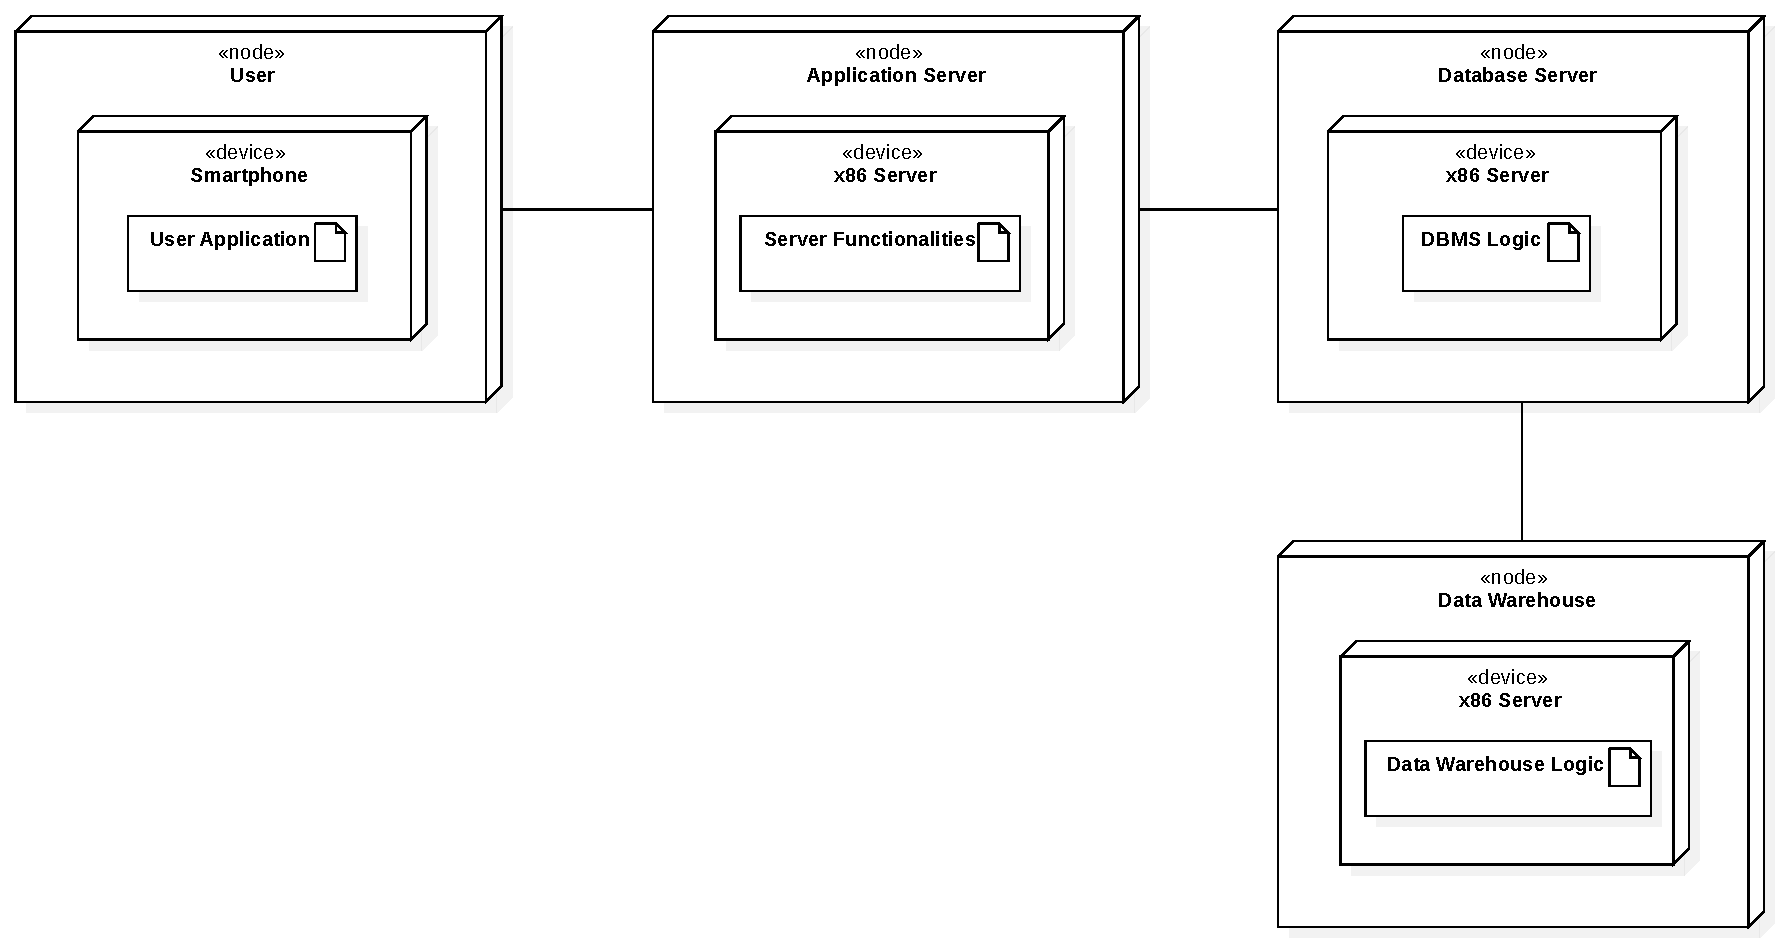
\includegraphics[width=\textwidth]{deployment_diagram}
\caption{Deployment diagram}
\label{fig:deployment_diagram}
\end{figure}

The presentation tier develops the user application, which only responsibility is
to present a user interface through which the user can communicate with the
application server. The application tier develops the application server, that
exploits all the application logic but does not contain any data, that, instead,
are stored in the database. The database is developed in the data tier, whose
purpose is also to split on different nodes the application database and the data
warehouse for data analysis and complex queries.

\end{document}